\section{Fourier Methods and Spectrograms}

Spectrograms have a long history, but were first properly used with music synthesis machine learning models at the start of the 21st century\cite{NoteOnsetDetection}.

The time-domain based audio signal was divided into equal length shorter periods. A Fast Fourier Transform (FFT) is then applied `to each segment, decomposing the signal at each of the timestep periods into their individual frequencies and corresponding amplitude. The complex values from the Fast Fourier Transform are complex values, giving spectrograms of frequency and phase.

A spectrogram is a graphical plot of the decomposition of sound using the \acrfull{STFT}. It consists of 2 plots frequency against time and phase against time. Each point of the plots is coloured in amplitude/intensity of the decomposed audio signal at that point in time.

The STFT is a sum of overlapped Fast Fourier Transforms (FFTs) of the audio signal. The sample is then divideded into overlapping frames of equal length known as the hamming window. The FFT is then applied to each frame of the audio signal. 

\subsection{Mel-Spectrograms}

Mel Spectrogrograsm are an adaptation of the spectrograms more suited to  sounds intended to be heard by humans. This is because Mel- Spectrograms have amplitude/sound intensity adjusted along a logarithmic scale such that graphical distances between frequencies sound the same distance as human hearing would detect them to be.

This enables machine learning models to learn how to produce audio sequences that sound more natural to a human listener.

\begin{figure}
    \centering
    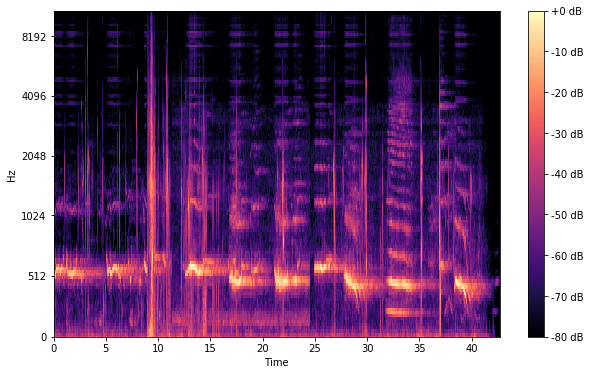
\includegraphics[width=0.8\textwidth]{literature_review/MelSpectrogram.png}
    \caption{An example of a  Mel Spectrogram showing the amplitude of different frequencies in a sound over time\cite{GettingToKnowTheMelSpectrogram}}
    \label{fig:spectrograms}
\end{figure}

There is no standardised formula for converting frequncy onto the mel logarhthmic scale as it is up to interpretation the adjustment level that is required for human hearing, though then most common formula is\cite{SpeechCommunication}:

\begin{equation}
    m = 2596 log(1 +  \frac{f}{700}) = 1127 ln (1 + \frac{f}{700})
\end{equation}

\subsection{Intepreting Phase}

The STFT is a complex function, however only the magnitude part is currently utilised by most models, and the phase part is discarded. Phase is key to the interpretation of musical sounds, without it syntheisized sounds can sound unnatural as signal information was discarded.

Success at interpreting the phase spectrogram to date has been limited. Most models simply choose to discard the phase part of the signal and make models purely off the frequency spectrogram. This is a problem as phase is a key part of audio making the image representation fully convertible back to audio, though it is difficult to work with for several reasons:

Firstly, phase appears to be random making it difficult to distinguish meaningful information from noise.

Secondly phase is a cyclic quality, cyclic qualities are harder to interpret than non-cyclic qualities as they are not continuous. One paper called GANSynth\cite{GANSynth} which attempts to overcome this problem. In this paper the difference in phase between individual timesteps of the spectrogram is calculated and $2\pi$ adjustments are made for when the phase wraps around. This difference in phase is called the instantaneous frequency and provides far more informative information than just the phase. Instantaneous frequency over harmonics for instance is expected to be constant.

\begin{figure}
    \centering
    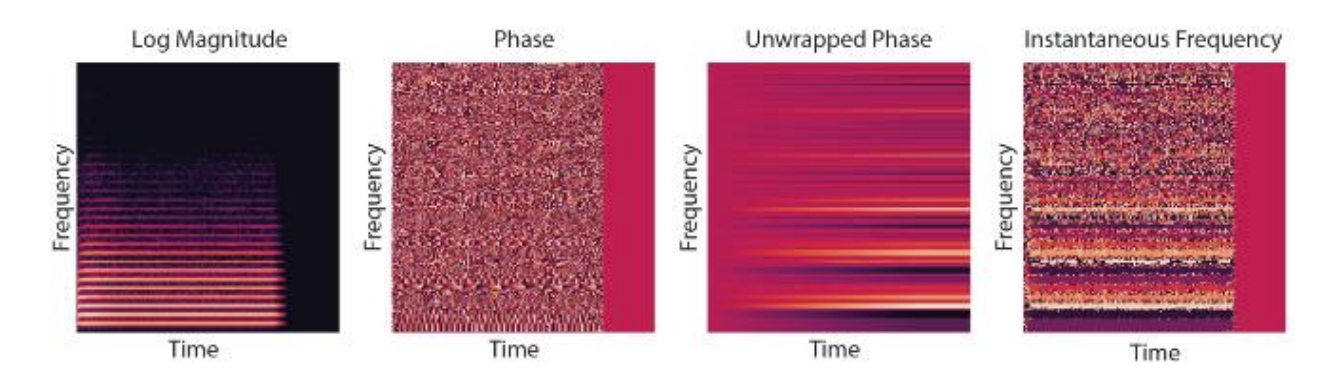
\includegraphics[width=0.8\textwidth]{literature_review/PhaseAdjustment.png}
    \caption{Unrwapping Spectrogram Phase: An illustration from the GANSynth paper of how the phase of a spectrogram is adjusted to make it more interpretable to a neural network\cite{GANSynth}}
    \label{fig:phase_unwrapping}
\end{figure}

\subsection{Spectrogram Evaluation}

Spectrogram based encoding for audio signal synthesis is currently the best method for encoding musical sounds due to their ease of use and the low level  control over signal information that does not hinder their interpretation (unlike raw waveform encoding). However they are not without problems (eg the discarding of phase information).

What makes spectgrogram based models useful is that conventional image processing models eg Convolutional Neural Networks or Recurrent Neural Networks can be used to process the spectrogram. This allows for a much more efficient representation of the audio signal and imaged based detection models are already fairly advanced.

Probably one of their defining advatages is they can be used to reconstruct the original audio signal from the spectrogram with the inverse Fourier Transform. If phase and magnitude spectrograms are used, the reconstructed audio signal will be almost identical to the original (phase matched).

Spectrograms are at the core of a significant number of recently published music synthesis models and papers, showing accademic relevance.

Models based on spectrograms, e.g. raw CNN based models are however limited and don't make use of biases in sound, for instance the tendancy of natural sounds to oscillate sinusoidally at harmonic frequencies.

Therefore spectrograms although useful cannot be used to directly synthesize audio signals, a further representation to help a model relate them to sound is required, for example \nameref{section:DDSP}.